\chapter[
	Proposition d'un \textit{Clustering Interactif}
]{
	Proposition d'un \textit{Clustering Interactif} pour assister la modélisation d'un jeu de données textuelles
}
\label{chapter:3-CLUSTERING-INTERACTIF}
	
	% RÉSUMÉ DES ÉPISODES PRÉCÉDENTS: LA MODELISATION C'EST COMPLIQUÉ !
	Dans le chapitre précédent, nous avons vu les points essentiels suivants :
	%
	\begin{leftBarImportantGreen}
		\begin{todolist}
			% Importance de la modélisation. Mais modélisation complexe. Donc organisation généralement en cycle.
			\item[\itemok] L'étape de modélisation est nécessaire pour définir les objectifs et les règles d'un projet d'annotation ;
			or cette étape rencontre de nombreux défis qui la rendant particulièrement laborieuse (\textit{complexité intrinsèque du phénomène, subjectivité des opérateurs, différences de comportements, ...}).
			ainsi, la modélisation est régulièrement révisée (cycle \texttt{MATTER}).
			% Conception de chatbot task-oriented correspond à ce problème : phénomène complexe, modélisation complexe, experts mal intégrés.
			\item[\itemok] La modélisation de textes en intentions pour entraîner un assistant conversationnel orienté par tâches n'échappe pas à ce constat, notamment à cause de la complexité du langage naturel, de la diversité d'intentions de dialogue à représenter, et de la pression sur le contrôle du comportement de l'assistant.
			% Besoins d'experts ; Interventions complexes ; Tâche pénible et couteuse.
			\item[\itemok] Dans un cadre industriel, des experts métiers sont responsables de la modélisation et de l'annotation des données spécifiques ou confidentielles de l'entreprise ;
			or ces interventions requièrent des compétences analytiques et techniques dont les experts métiers ne disposent pas forcément ;
			de ce fait, la manipulation d'une modélisation abstraite de leurs connaissances est alors vécue comme une tâche pénible, nécessitant un grand nombre de formations et organisée sous la forme d'ateliers en mode essai-erreur.
		\end{todolist}
	\end{leftBarImportantGreen}
	
	% ANNONCE DU BUT DU CHAPITRE: MA CONTRIBUTION !
	Dans cette partie, nous cherchons une alternative à cette organisation traditionnelle, et nous proposerons une méthodologie d'annotation basée sur un \texttt{Clustering Interactif} visant à remplir un double objectif :
	%
	\begin{leftBarImportantRed}
		\begin{todolist}
			% 1. Efficacité de création du trainset.
			\item Permettre d'assister la modélisation et l'annotation des données pour créer plus efficacement une base d'apprentissage destinée à la classification d'intentions d'un assistant conversationnel ;
			% 2. Efficacité d'intervention d'un expert.
			\item Redéfinir les tâches et les objectifs des différents acteurs afin de rester au plus proche de leurs compétences réelles, particulièrement en ce qui concerne l'intervention des experts métiers du projet.
		\end{todolist}
	\end{leftBarImportantRed}
	
	% Référence articles.
	\begin{leftBarInformation}
		Cette proposition de méthode a été l'objet d'une présentation à la conférence \texttt{EGC (Extraction et Gestion des Connaissances)}~(\cite{schild-etal:2021:conception-iterative-semisupervisee}), et d'une extension dans le journal \texttt{IJDWM (International Journal of Data Warehousing and Mining)}~(\cite{schild-etal:2022:iterative-semisupervised-design}).
		Nous reprenons ici certains des éléments présentés avec quelques détails supplémentaires.
	\end{leftBarInformation}

	% TABLE DES MATIÈRES DU CHAPITRE
	\minitoc


	%%%%%--------------------------------------------------------------------
	%%%%% Section 3.1: Intuitions à l'origine d'un \textit{Clustering Interactif}.
	%%%%%--------------------------------------------------------------------
	%\newpage
	%\vspace{2cm}
	\section{Intuitions à l'origine d'un \textit{Clustering Interactif}}
\label{section:3.1-INTUITIONS-ORIGINES}

	Tout d'abord, détaillons trois intuitions qui nous ont permis de concevoir notre méthodologie d'annotation.
	
	
	%%%
	%%% Subsection 3.1.1. Utiliser une approche non-supervisées pour créer une modélisation.
	%%%
	\subsection{Utiliser une approche non-supervisées pour créer une modélisation}
	\label{section:3.1.1-INTUITIONS-ORIGINES-NON-SUPERVISEES}
	
		%%% Possibilité d'utilisé des regroupements non supervisés.
		Dans le but d'assister la phase de modélisation des données, une piste intéressante revient à déléguer cette tâche à la machine.
		En effet, grâce à une \textbf{classification non-supervisés (\textit{clustering})}, un algorithme peut regrouper les données en fonction de leur similarité intrinsèque et ainsi suggérer une modélisation intentions.
		%%% Quelques exemples communs: KMeans, Hiérarchique, Spectral, DBScan, Affinity propagation, ...
		Plusieurs algorithmes et méthodes connus peuvent être utilisés :
		
		\begin{itemize}
			% KMeans.
			\item Le \textbf{\textit{clustering} \texttt{KMeans}} (\cite{macqueen:1967:methods-classification-analysis}) :
			Cette méthode se repose sur la minimisation de l'inertie intra-classes en attribuant chaque donnée au barycentre de \textit{cluster} le plus proche.
			Cette approche est l'une des plus répandues en raison de sa simplicité et de sa rapidité de calcul ;
			% Hiérarchique.
			\item Le \textbf{\textit{clustering} hiérarchique} (\cite{murtagh-contreras:2012:algorithms-hierarchical-clustering}) :
			Cette méthode revient à fusionner itérativement les données les plus similaires dans un nouveau \textit{cluster}.
			Plusieurs liens de similarité peuvent être implémentés (\textit{le lien \texttt{single} fusionnant les deux \textit{clusters} ayant les frontières les plus proches, le lien \texttt{complete} fusionnant les deux \textit{clusters} ayant les frontières opposées les plus proches, le lien \texttt{average} fusionnant les deux \textit{clusters} ayant les barycentres les plus proches et le lien \texttt{ward} fusionnant les deux \textit{clusters} qui donneront le prochain \textit{cluster} le plus compact}) ;
			% Spectral.
			\item Le \textbf{\textit{clustering} spectral} (\cite{ng-etal:2002:spectral-clustering-analysis}) :
			Cette méthode consiste à modéliser la matrice de similarité entre les données par ses vecteurs propres puis de regrouper ces derniers à l'aide d'un \texttt{KMeans}.
			Cette approche permet d'obtenir des \textit{clusters} aux formes complexes ;
			% DBScan.
			\item Le \textbf{\textit{clustering} \texttt{DBScan}} (\cite{ester-etal:1996:densitybased-algorithm-discovering}) :
			Cette méthode utilise la densité de données dans l'espace pour identifier des regroupements.
			Cette approche permet de découvrir des \textit{clusters} aux formes complexes si leur densité est suffisante.
			\item ...
		\end{itemize}
		
		%%% Cependant, il y a des limites.
		Cependant, ces algorithmes non-supervisés font régulièrement face à un ensemble de difficultés qui pénalisent leur utilisations.
		En effet, ces méthodes ont souvent du mal à traiter des données de grandes dimensionnalités ou en grand nombre (\cite{steinbach-etal:2004:challenges-clustering-high}), la présence de bruits peut rapidement perturber le fonctionnement d'un algorithme (\cite{yang-wang:2004:competitive-algorithms-clustering}), et certains \textit{clusters} aux géométries complexes peuvent être difficiles à identifier (\cite{kriegel-etal:2011:density-based-clustering}).
		De plus, le choix de certains hyperparamètres de ces méthodes n'est pas toujours simple, surtout en ce qui concerne le nombre de clusters, la méthode d'initialisation ou la mesure de distance à utiliser (\cite{agarwal-etal:2011:issues-challenges-tools}).
		Enfin, toutes ses difficultés se retrouvent dans le traitement du langage naturel, notamment à cause de la taille de vocabulaire important, de la présence de nombreux bruits et de la vaste diversité et complexité de thématiques pouvant y être abordés.
		\begin{leftBarInformation}
			La revue de \cite{xu-tian:2015:comprehensive-survey-clustering} détaille plusieurs algorithmes de \textit{clustering}, en fonction de leurs forces et faiblesses sur les points mentionnés ci-dessus.
		\end{leftBarInformation}
		
		% Conclusion : souvent jugés peu pertinents par les experts métiers.
		Ainsi, toutes ces limites étayent le fait qu'\textbf{un résultat brut d'une classification non supervisées est généralement perçu comme peu pertinent par les experts métiers}.
		Il est donc nécessaire d'introduire une intervention humaine dans le processus pour guider le fonctionnement d'un algorithme de \textit{clustering}.
		
	
	%%%
	%%% Subsection 3.1.2. Corriger l'approche non-supervisée avec une annotation de contraintes.
	%%%
	\subsection{Corriger l'approche non-supervisée avec une annotation de contraintes}
	\label{section:3.1.2-INTUITIONS-ORIGINES-SEMI-SUPERVISEES}
	
		%%% Proposition d'ajouts de contraintes pour corriger un \textit{clustering}.
		Une variante aux approches non-supervisées consiste à demander à un humain certaines informations nécessaires à leur amélioration nous considérons donc les \textbf{approches semi-supervisées}.
		Une manière efficace d'introduire les connaissances d'un expert dans le processus est l'ajout de contraintes.
		
		%%% Plusieurs types de contraintes.
		\cite{lampert-etal:2018:constrained-distance-based} rappelle qu'il peut y avoir deux types de contraintes :
		\begin{itemize}
			\item les \textbf{contraintes sur les données} : on parle alors principalement des contraintes binaires \texttt{MUST-LINK} et \texttt{CANNOT-LINK} décrivant si deux données doivent ou ne doivent être dans un même clusters (\cite{wagstaff-cardie:2000:clustering-instancelevel-constraints})
			\item les \textbf{contraintes sur les \textit{clusters}} : ces contraintes peuvent concerner le nombre de \textit{clusters} à trouver, leur taille minimale ou maximale, la distance minimale de séparation de leurs frontières, ...
		\end{itemize}
		
		% Nous choississons plutôt les contraintes sur les données.
		Bien que d'autres méthodes permettent d'insérer des contraintes (heuristiques non-supervisées, transferts de connaissances préalables), nous nous concentrons ici sur l'ajout manuel par un expert.
		Comme cet expert n'a a priori pas de connaissances techniques ou analytiques, ce dernier aurait du mal à manipuler des contraintes sur les \textit{clusters}.
		Toutefois, ses connaissances métiers lui permettent de caractériser facilement la similarité entre deux données, et donc de décrire des contraintes de type \texttt{MUST-LINK} et \texttt{CANNOT-LINK} en répondant à la question : \textguillemets{\textit{est-ce les deux données traite du même cas d'usage ?}}.
		
		\begin{leftBarAuthorOpinion}
			La pierre angulaire de la méthode que nous proposons en \textsc{Section~\ref{section:3.2-DESCRIPTION-THEORIQUE}} repose notamment sur le fait qu'il est difficile pour un expert métier de classer une question suivant une modélisation abstraite prédéfinie : cela l'éloigne de ses compétences métiers initiales, nécessite en contre-partie de nombreuses formations, et introduit de nombreuses erreurs d'annotations.
			De fait, il semble plus adéquat de demander à l'expert métier de discriminer deux questions sur la base de leurs similarité de cas d'usage métier.
		\end{leftBarAuthorOpinion}
		
		
		%%% Quelques exemples communs : COP KMeans, Hiérarchique, SPEC Spectral, C-DBScan, ...
		Parmi les algorithmes de \textit{clustering} sous contraintes connus, nous disposons des adaptations suivantes :
		
		\begin{itemize}
			% KMeans.
			\item Le \textbf{\textit{clustering} \texttt{KMeans} sous contraintes} comme \texttt{COP-KMeans} (\cite{wagstaff-etal:2001:constrained-kmeans-clustering}) :
			Dans cette version, l'attribution d'une donnée se fait au \textit{cluster} dont le barycentre est le plus proche et où aucune contraintes n'est violée.
			Cette adaptation est relativement simple à mettre en oeuvre, mais elle peut mener à des cas de blocage où plus aucun \textit{cluster} n'est accessible à cause de violation de contraintes (il est possible d'adapter l'algorithme en créant un nouveau \textit{cluster}) ;
			% Hiérarchique.
			\item Le \textbf{\textit{clustering} hiérarchique sous contraintes} (\cite{davidson-ravi:2005:agglomerative-hierarchical-clustering}) :
			Dans cette version, les données liées par des contraintes \texttt{MUST-LINK} sont d'abord fusionnées, puis le processus agglomératif commence en prenant garde de ne pas fusionner des \textit{clusters} ayant des contraintes \texttt{CANNOT-LINK} entre eux.
			Cette adaptation est très simple à mettre en oeuvre car il suffit d'adapter le calcul de distance entre \textit{clusters} ;
			% Spectral.
			\item Le \textbf{\textit{clustering} spectral sous contraintes} (\cite{kamvar-etal:2003:spectral-learning}) :
			Dans cette version, les coefficients de la matrice de similarité sont forcés à $0$ (respectivement $1$) si deux données sont liées par une contrainte \texttt{CANNOT-LINK} (respectivement \texttt{MUST-LINK}).
			Cette adaptation demande peu d'effort pour être mise en oeuvre, mais des modifications aussi drastiques de la matrice de similarité peut entraîner des changements imprévisibles de comportements ;
			% DBScan.
			\item Le \textbf{\textit{clustering} \texttt{DBScan} sous contraintes} comme \texttt{C-DBScan} (\cite{ruiz-etal:2010:densitybased-semisupervised-clustering}) :
			Dans cette version, la densité des données ainsi que les contraintes \texttt{CANNOT-LINK} sont utilisées pour identifier des clusters locaux qui seront ensuite fusionnés à l'aide des contraintes \texttt{MUST-LINK}
			Cette adaptation est plus compliquée à réaliser car elle change légèrement le fonctionnement interne d'exploration de la densité de l'espace de données.
			\item ...
		\end{itemize}
		
		Ces algorithmes de \textit{clustering} sous contraintes sont ainsi plein de potentiels : ils sont en effet capable de tirer parti de la similarité intrinsèque des données et des contraintes judicieusement placées de l'expert pour segmenter les données de manière adéquate et ainsi proposer une modélisation pertinente.
		\begin{leftBarExamples}
			On peut citer \cite{lampert-etal:2019:constrained-distance-based} où l'annotation de contraintes par un expert d'identifier efficacement dans objets dans une image satellite.
		\end{leftBarExamples}
		
		%%% Cependant, ils peuvent demander énorméments de contraintes : N^2 !
		Cependant, pour un jeu de données de taille $N$, il y a $N^2$ possibilités de contraintes à ajouter.
		L'estimation du placement des contraintes les plus appropriées et les plus efficaces pour corriger le \textit{clustering} semble donc être un problème \texttt{NP}-complexe.
		De plus, si ce choix peut être visuel pour des images (comme dans l'exemple cité ci-dessus), il ne l'est pas pour des données textuelles dont la diversité et la complexité sont difficiles à appréhender.
		Il est donc important d'assister l'expert métier à disposer ses contraintes afin de maximiser son impact dans la correction du \textit{clustering}.
		
	
	%%%
	%%% Subsection 3.1.3. Tirer parti des avantages de l'apprentissage actif pour optimiser les interactions Homme/machine.
	%%%
	\subsection{Tirer parti des avantages de l'apprentissage actif pour optimiser les interactions Homme/machine}
	\label{section:3.1.3-INTUITIONS-ORIGINES-APPRENTISSAGE-ACTIF}
	
		% Utiliser l'apprentissage actif.
		Une dernière piste intéressante est celle de l'apprentissage actif (\textit{active learning}, voir \cite{settles:2010:active-learning-literature}) : celle-ci prône les interactions Homme/machine comme moyen d'atteindre un objectif qu'aucun en peut atteindre séparément.
		% Liste d'interactions possibles avec le résultat, avec les hyperparamètres, avec des initaitives de la machine, ...
		\cite{bae-etal:2021:interactive-clustering-comprehensive} liste par exemple un ensemble d'interactions possibles avec un algorithme de \textit{clustering} : celles-ci peuvent concerner la manipulation et l'adaptation des résultats, l'adaptation des hyperparamètres des algorithmes, mais aussi des initiatives de la machine pour préparer la réalisation d'une tâche.
		
		% Nous sommes intéresser par la sélection optimale de contraintes à annoter
		Dans notre cas, nous nous intéressons en particulier aux initiatives de la machines pour identifier la liste des contraintes à annoter pour corriger ou confirmer efficacement un résultat de \textit{clustering}.
		Cela peut se faire par exemple à l'aide d'une heuristique sélectionnant les parties les moins sûres de la segmentation.
	
	%%%
	%%% Conclusion.
	%%%
	\begin{leftBarSummary}
		Dans cette partie, nous avons exposés les intuitions suivantes :
		\begin{todolist}
			% Pression sur la qualité.
			\item[\itemok] La phase de modélisation des données peut être déléguée à la machine en employant des algorithmes de classification non-supervisée (\textit{clustering}) ;
			\item[\itemok] Pour corriger le fonctionnement d'un algorithme de \textit{clustering} et ainsi améliorer la pertinence de ses résultats, l'expert peut ajouter des contraintes binaires sur les données (\texttt{MUST-LINK} et \texttt{CANNOT-LINK}, \textit{clustering} sous contraintes) ;
			\item[\itemok] Dans le but d'ajouter des contraintes de manière efficace, il est possible d'interagir avec la machine afin de maximiser l'impact de l'intervention de l'expert (\textit{active learning}).
		\end{todolist}
	\end{leftBarSummary}


	%%%%%--------------------------------------------------------------------
	%%%%% Section 3.2: Description théorique de notre \textit{Clustering Interactif}
	%%%%%--------------------------------------------------------------------
	%%% TODO\newpage
	%\vspace{2cm}
	\section{Description de notre \textit{clustering} interactif.}
\label{section:3.2-DESCRIPTION-THEORIQUE}

	Sur la base des intuitions que nous venons de détailler, nous proposons la méthode suivante dans le but d'assister la modélisation et l'annotation d'une collecte de données brutes en une base d'apprentissage nécessaire à l'entraînement d'un assistant conversationnel.
	
	%%%
	%%% Subsection 3.2.1. Description générale.
	%%%
	\subsection{Description générale}
	\label{section:3.2.1-DESCRIPTION-THEORIQUE-GENERALE}
	
		% Présentation succinte.
		\textbf{Notre méthode d'annotation}, que nous appelons \textguillemets{\texttt{Clustering Interactif}}, \textbf{repose sur l'alternance successive entre deux phases clefs} (voir \textsc{Figure~\ref{figure:3.2-CLUSTERING-INTERACTIF}}) :
		\begin{itemize}
			\item[\(\bullet\)] une phase d'\textbf{annotation de contraintes}
			par un expert permettant de caractériser la similarité entre deux données suivant leur cas d'usage métier ;
			\item[\(\bullet\)] une phase de \textbf{segmentation automatique} des données
			par une machine sur la base de la proximité sémantique des données et des contraintes précédemment annotées.
		\end{itemize}
		
		% Objectif recherché
		L'objectif recherché en associant ces deux phases est de \textbf{créer un cercle vertueux pour améliorer itérativement la qualité de la base d'apprentissage} en cours de construction.
		En effet, à chaque itération, l'expert métier obtiendra une proposition de segmentation des données qu'il pourra raffiner dans le but de corriger le fonctionnement de la machine et ainsi d'obtenir une segmentation plus pertinente à l'itération suivante.
		
		% Figure.
		\begin{figure}[!htb]
			\centering
			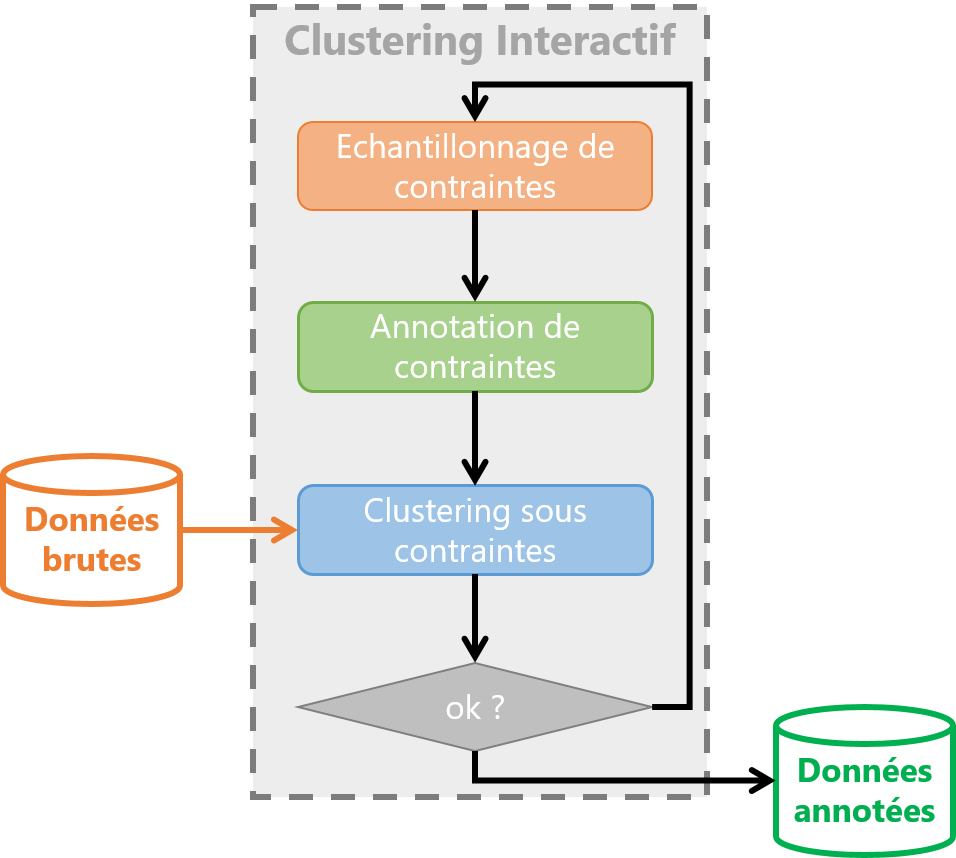
\includegraphics[width=0.95\textwidth]{figures/interactive-clustering-architecture-sequentielle}
			\caption{
				Schéma illustrant l'architecture du \textit{clustering} interactif.
				La boucle principale enchaîne un échantillonnage de couples de données, une annotation de contraintes, et un \textit{clustering} sous contraintes.
			}
			\label{figure:3.2-CLUSTERING-INTERACTIF}
		\end{figure}
	
	
	%%%
	%%% Subsection 3.2.2. Description détaillée.
	%%%
	\subsection{Description détaillée}
	\label{section:3.2.2-DESCRIPTION-THEORIQUE-DETAILLEE}
	
		% Pseudo code.
		L'\textsc{Algorithme~\ref{algorithm:3.2-CLUSTERING-INTERACTIF}} décrit formellement notre proposition de \texttt{Clustering Interactif} que nous détaillons ci-dessous.
		\begin{algorithm}
			\KwData{données non segmentées}
			\KwIn{budget à disposition}
			%
			\textbf{initialisation}: créer une liste vide de contraintes \;
			\textit{optionnel}: évaluer les hyper-paramètres de la segmentation automatique \;
			\textbf{segmentation initial}: regrouper les données par similarité \;
			\Repeat{segmentation satisfaisante OU budget épuisé}{
				\textit{optionnel}: évaluer les hyper-paramètres de l'échantillonnage \;
				\textbf{échantillonnage}: sélectionner une partie de la segmentation à corriger \;
				\textbf{annotation}: corriger la segmentation en ajoutant des contraintes sur l'échantillon \;
				\textit{optionnel}: ré-évaluer les hyper-paramètres de la segmentation automatique \;
				\textbf{segmentation}: regrouper les données par similarité avec les contraintes \;
				\textbf{validation}: estimer la pertinence et la stabilité de la segmentation \;
				\textbf{coûts}: estimer le budget restant et les coûts restant à investir \;
			}
			\textbf{interprétation}: trier et nommer les clusters pour les exploiter \;
			%
			\KwResult{données segmentées (i.e. base d'apprentissage)}
			%
			\caption{\textit{
				Description en pseudo-code de la méthode d'annotation proposée employant le \textit{clustering} interactif.
			}}
			\label{algorithm:3.2-CLUSTERING-INTERACTIF}
		\end{algorithm}
		
		% Description de l'initialisation.
		Pour l'\textbf{initialisation} de la méthode (cf. \textsc{Algorithme~\ref{algorithm:3.2-CLUSTERING-INTERACTIF}}, \textit{lignes 1 à 3}), nous définissons une liste vide de contraintes : tout au long du processus, nous y ajoutons les contraintes annotées par l'expert grâce à ses connaissances métiers (nous entrerons en détails en décrivant la phase d'annotation).
		Il faut aussi une première segmentation des données par la machine : celle-ci se réalise par l'exécution d'un algorithme de \textit{clustering}.
		Nous estimons qu'il n'est pas du ressort de l'expert métier de choisir le réglage de l'algorithme de \textit{clustering} et ses hyper-paramètres.
		Ces derniers pourront être déterminés par un \textit{data scientist} en fonction du problème à traiter ou laissés par défaut.
		Il est à noter que cette première segmentation des données est réalisée sans bénéficier de la connaissance de l'expert, il est donc peu probable que le résultat soit pertinent à ce stade.
		
		% Description de l'échantillonnage.
		Nous entrons dans le coeur de la boucle itérative par la phase d'\textbf{échantillonnage} (cf. \textsc{Algorithme~\ref{algorithm:3.2-CLUSTERING-INTERACTIF}}, \textit{lignes 5 et 6}).
		Comme mentionné au préalable, savoir quelles contraintes ajouter pour corriger efficacement le \textit{clustering} est un problème NP-difficile (le nombre de possibilités croît proportionnellement au carré du nombre de données).
		De plus, l'intervention d'experts est chiffrée et représente en général une partie des coûts à investir dans un projet (voir \textsc{Section~\ref{section:2.3.2.C-DEFIS-ANNOTATION-ASPECT-COMPLEXITE-COUTS}}).
		Il est donc inconcevable de laisser un expert métier annoter des contraintes "seul" et "au hasard".
		Ainsi, pour optimiser ses interventions, il convient de déterminer là où l'expert aura le plus d'impact lors de sa transmission de connaissances.
		C'est pourquoi la phase d'échantillonnage est primordiale dans la méthode proposée : Nous proposons d'y sélectionner des couples de données sur la base de leur similarité, de leur segmentation ou encore de leurs relations avec d'autres données déjà liées par des contraintes.
		
		% Description de l'annotation.
		Sur la base de cet échantillon, l'expert peut entamer son étape d'\textbf{annotation de contraintes} (cf. \textsc{Algorithme~\ref{algorithm:3.2-CLUSTERING-INTERACTIF}}, \textit{ligne 7}).
		Pour alléger la charge d'annotation, nous avons décidé de discriminer les données de l'échantillon par des contraintes binaires simples : \texttt{MUST-LINK} et \texttt{CANNOT-LINK}.
		Ces contraintes représentent respectivement la similitude ou la différence entre deux données, et seront utilisées pour regrouper ou séparer certaines données dans la prochaine segmentation.
		En fonction de l'orientation du projet et afin de rester au plus proche des compétences réelles de l'expert, la formulation de l'énoncer d'annotation doit être judicieusement définie : par exemple, les contraintes peuvent représenter une similitude
		sur la thématique concernée \footnote{
			Exemples de thématiques : \textit{crédit} vs. \textit{assurance} ; \textit{sport} vs. \textit{culture}, ...
		}, sur l'action désirée \footnote{
			Exemples d'actions : \textit{souscrire} vs. \textit{résilier} ; \textit{activer} vs. \textit{désactiver} ; \textit{s'informer} vs. \textit{réaliser}, ...
		}, ou encore sur le besoin de l'utilisateur \footnote{
			Exemple de besoins : \textit{souscrire un crédit} vs. \textit{souscrire une assurance} ; \textit{s'informer en sport} vs. \textit{s'informer en culture}, ...
		}.
		On notera que des incohérences peuvent s'introduire, ayant pour conclusions de devoir à la fois considérer comme similaires et différentes deux données : ces incohérences peuvent être détecter grâce à aux propriétés de transitivités des contraintes (voir la gestion des conflits en \textsc{Annexe~\ref{section:C.1.2-DESCRIPTION-IMPLEMENTATION-INTERACTIVE-CLUSTERING-GESTION-DES-CONTRAINTES}}).
		
		% Description du clustering.
		Pour finir, la dernière phase de cette boucle est composée d'une nouvelle \textbf{segmentation} des données (cf. \textsc{Algorithme~\ref{algorithm:3.2-CLUSTERING-INTERACTIF}}, \textit{lignes 8 et 9}).
		Cette segmentation devra respecter les contraintes préalablement définies par l'expert, nous nous tournons donc vers l'utilisation d'un \textit{clustering} sous contraintes.
		Au fur et à mesure des itérations, de plus en plus de contraintes seront ajoutées pour corriger le \textit{clustering}. ainsi, au bout d'un certain nombre d'itérations, la segmentation des données reflétera la vision que l'expert aura voulu transmettre.
		Comme précédemment, nous estimons qu'il n'est pas du ressort de l'expert métier de choisir de l'algorithme de \textit{clustering} et ses hyper-paramètres.
		Ces derniers pourront être déterminés par un \textit{data scientist} en fonction du problème à traiter, estimés en fonction de l'itération et des contraintes disponibles, ou laissés par défaut.
		
		% Description de l'évaluation.
		Comme la méthode est itérative, il faut pouvoir estimer des \textbf{cas d'arrêt} (cf. \textsc{Algorithme~\ref{algorithm:3.2-CLUSTERING-INTERACTIF}}, \textit{lignes 10 à 12}).
		Le cas d'arrêt le plus évident n'est pas technique mais relatif aux coûts investis dans l'opération : si le projet n'a plus de budget dédié à l'annotation, il faudra créer la base d'apprentissage avec le résultat à disposition, quel que soit la pertinence de la segmentation obtenue sur les données.
		Ce cas d'arrêt par défaut peut malheureusement être synonyme d'échec pour le projet si les résultats sont inexploitables.
		D'autres cas d'arrêts peuvent être envisagés en fonction de la qualité ou de la pertinence de la segmentation.
		D'une part, nous pouvons comparer l'évolution de la segmentation des données : si les segmentations sont similaires sur plusieurs itérations, il est possible que la modélisation atteint un optimum local ou un palier de performance.
		D'autre part, nous pouvons aussi comparer l'évolution de l'accord entre la segmentation obtenue et l'annotation de l'expert : en effet, si l'expert ne contredit plus la répartition proposée des données, il est probable que sa vision et la vision de la machine aient convergé.
		Dans les deux cas, l'analyse de l'expert métier reste nécessaire pour valider si la modélisation des données est pertinente ou si elle comporte encore des incohérences à corriger.

		% Description de l'évaluation.
		Lorsque la boucle itérative est finie, nous avons à disposition une segmentation des données qui a été corrigé par un expert et qui reflète ses connaissances métier.
		La dernière étape consiste alors à \textbf{interpréter} ces \textit{clusters} pour pouvoir les exploiter (cf. \textsc{Algorithme~\ref{algorithm:3.2-CLUSTERING-INTERACTIF}}, \textit{ligne 13}).
		Cela commence par leur attribuer un nom au lieu de leur identifiant technique, de les définir en les rapprochant d'un cas d'usage métier, et éventuellement de les raffiner manuellement en supprimant certaines données aberrantes.
		
		% Exemple abstrait.
		\begin{leftBarExamples}
			La \textsc{Figure~\ref{3.2-CLUSTERING-INTERACTIF-EXEMPLE}} déroule l'initialisation et la première itération de la méthode sur un exemple fictif.
			Nous pouvons constater qu'entre les images \textbf{(2)} et \textbf{(5)}, la segmentation des données à évoluée grâce à l'introduction de contraintes.
		
			\begin{figure}[H]
				\centering
				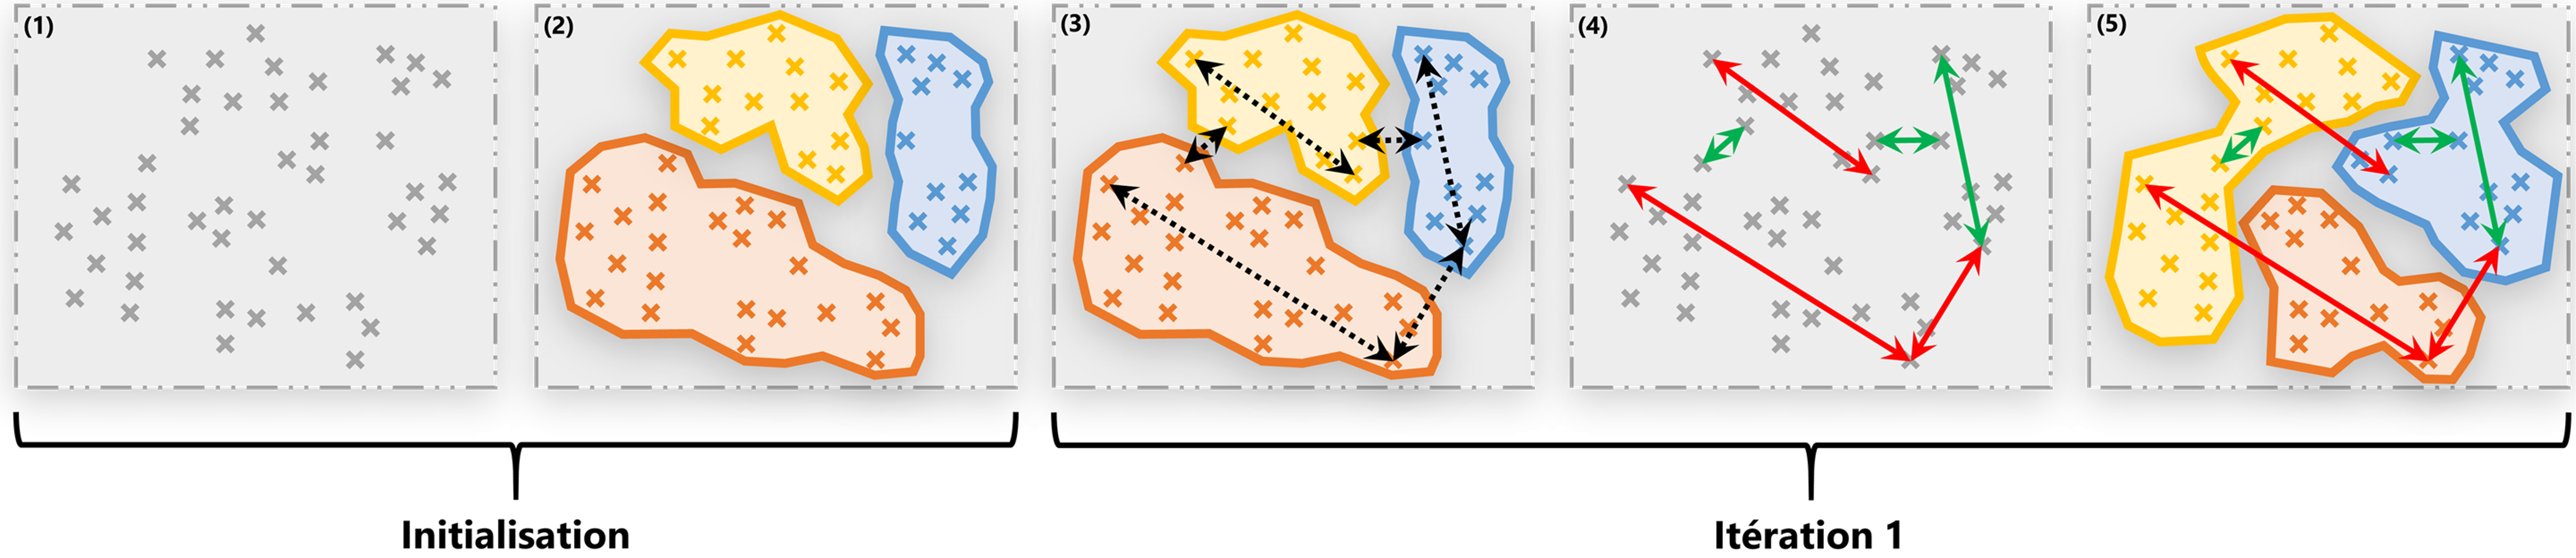
\includegraphics[width=0.95\textwidth]{figures/example-iteration-clustering-interatif}
				\caption{
					Exemple d'une itération de \textit{clustering} interactif. \\
					Lors de l'initialisation,
					\textbf{(1)} correspond au jeu de données brut,
					et \textbf{(2)} correspond à une première segmentation des données en $3$ \textit{clusters}.
					Lors de l'itération $1$ :
					\textbf{(3)} correspond à un exemple d'échantillonnage de $6$ contraintes représentées par les flèches en pointillées,
					\textbf{(4)} correspond à la caractérisation de ces $6$ contraintes par des liens \texttt{MUST-LINK} en vert et \texttt{CANNOT-LINK} en rouge,
					et \textbf{(5)} correspond à la nouvelle segmentation des données en $3$ \textit{clusters} respectant les $6$ contraintes annotées.
					La prochaine itération se poursuivra par un nouvel échantillonnage de contraintes.
				}
				\label{3.2-CLUSTERING-INTERACTIF-EXEMPLE}
			\end{figure}
		\end{leftBarExamples}
	

	
	%%%
	%%% Subsection 3.2.3. Description techniques et implémentation.
	%%%
	\subsection{Description techniques et implémentation}
	\label{section:3.2.3-DESCRIPTION-TECHNIQUE-IMPLEMENTATION}
	
		% Généralités.
		Au cours de ce doctorat, nous avons réalisé une implémentation en Python de notre \textit{clustering interactif}.
		Celle-ci est répartie en trois librairies :
		\begin{enumerate}
			% cognitivefactory-interactive-clustering
			\item \texttt{cognitivefactory-interactive-clustering} \footnote{
				\texttt{cognitivefactory-interactive-clustering}: la page de documentation technique de cette librairie est disponible ici : \url{https://cognitivefactory.github.io/interactive-clustering/}
			} (\cite{schild:2022:cognitivefactory-interactiveclustering}), regroupant les gestions de données, la gestion des contraintes, les algorithmes de \textit{clustering} sous contraintes et les algorithmes d'échantillonnage implémentés ;
			% cognitivefactory-features-maximization-metric
			\item \texttt{cognitivefactory-features-maximization-metric} \footnote{
				\texttt{cognitivefactory-features-maximization-metric}: la page de documentation technique de cette librairie  est disponible ici : \url{https://cognitivefactory.github.io/features-maximization-metric/}
			} (\cite{schild:2023:cognitivefactory-featuresmaximizationmetric}), disposant d'une méthode de sélection des patterns linguistiques pertinents (composantes principales) d'un jeu de données, utilisée pour l'analyse de pertinence d'un résultat de \textit{clustering} ;
			% cognitivefactory-interactive-clustering-gui
			\item \texttt{cognitivefactory-interactive-clustering-gui} \footnote{
				\texttt{cognitivefactory-interactive-clustering-gui}: la page de documentation technique de cette librairie  est disponible ici : \url{https://cognitivefactory.github.io/interactive-clustering-gui/}
			} (\cite{schild-etal:2022:cognitivefactory-interactiveclusteringgui}), encapsulant les algorithmes précédents et intégrant la logique de la méthode dans une application web.
		\end{enumerate}
		
		


	%%%%%--------------------------------------------------------------------
	%%%%% Section 3.3: Espoirs portés sur la méthode proposée.
	%%%%%--------------------------------------------------------------------
	%\newpage
	%\vspace{2cm}
	\section{Perspectives portées par la méthode proposée.}
\label{section:3.3-PERSPECTIVES-METHODE}

	% Rappel de la proposition.
	Nous avons proposé une méthodologie d'annotation basée sur une interaction entre l'Homme et la Machine dans le but de soulager l'expert métier dans son intervention.
	
	% Annonce des espoirs.
	Grâce à une telle approche, nous pouvons espérer que :
	\begin{todolist}
		\item Les experts métiers n'auront désormais plus besoin de bagages analytiques ou techniques pour intervenir dans un projet d'annotation ;
		\item Les experts métiers pourront désormais participer à la modélisation d'une base d'apprentissage en ayant des discussions pragmatiques sur les cas d'usages des données manipulées ;
		\item Une telle méthodologie d'annotation permettra d'obtenir efficacement une base d'apprentissage stable et pertinente pour entraîner une modèle de classification d'intention ;
		\item Une telle méthodologie d'annotation sera réaliste en terme de délais et d'investissement financier.
	\end{todolist}
	
	% Transition au chapitre 4.
	Nous allons explorer diverses pistes pour confirmer ou infirmer ces perspectives dans le \textsc{Chapitre~\ref{chapter:4-ETUDES}}, et nous détaillerons nos conclusions dans un guide d'utilisation qui sera présenté dans le \textsc{Chapitre~\ref{chapter:5-GUIDE}}.